\chapter{Conclusion}

\subsection{Future Work}
For further developments of the project, it could be interesting to take into consideration also the sentiment analysis.
This can be done by studying the lyrics of the songs and analyzing the sentiment of the lyrics, as it was done in the literature review. 
Finding out if a happy song is more keen to be popular than a sad song could be interesting.\\
Sentiment analysis could also be done on the reviews of the songs,
that could be done for example by analyzing what people write about a specific song or a specific artist. This could be done by getting the tweets that contain the name of the artist or the song and then analyze the sentiment of the tweets. Also the most important music magazines could be analyzed to see if the reviews of the songs are positive or negative and how this affects the popularity of the song.\\
All this information can be used to improve the model.\\
Another interesting thing to do is to improve the User Interface of the application. The application could be improved by adding more features, like the possibility to search for a specific song and see its popularity, or the possibility to see the most popular songs of a specific artist.\\



\subsection{Conclusion}
In general, finding the most popular songs is a very difficult task. The popularity of a song is influenced by many factors and it is not easy to predict it. 
This project has shown that it is possible to predict the popularity of a song with a good accuracy, which could help a lot in the music industry, but it could be improved.\\
The algorithms used in this project are proved to be more accurate than the ones used in the state of the art. In the state of art the more accurate algorithm is the Logistic Regression, which has an accuracy of 0.52, while in this project it is the Random Forests with an accuracy of 0.85.\\
They both agreed on the fact that the most important feature is in general danceability, but as we went further in the research to find the most important features for different regions of the world it resulted that not all of them have danceability as the most important feature.\\
Furthermore, we highlighted that the most important features for the popularity of a song are different for different regions of the world. This shows that there are cultural differences also in music and that the same song could be popular in one region and not in another.\\

%change images: use random forests\\
\begin{figure}[H]
    \centering
    \begin{minipage}{0.45\textwidth}
        \centering
        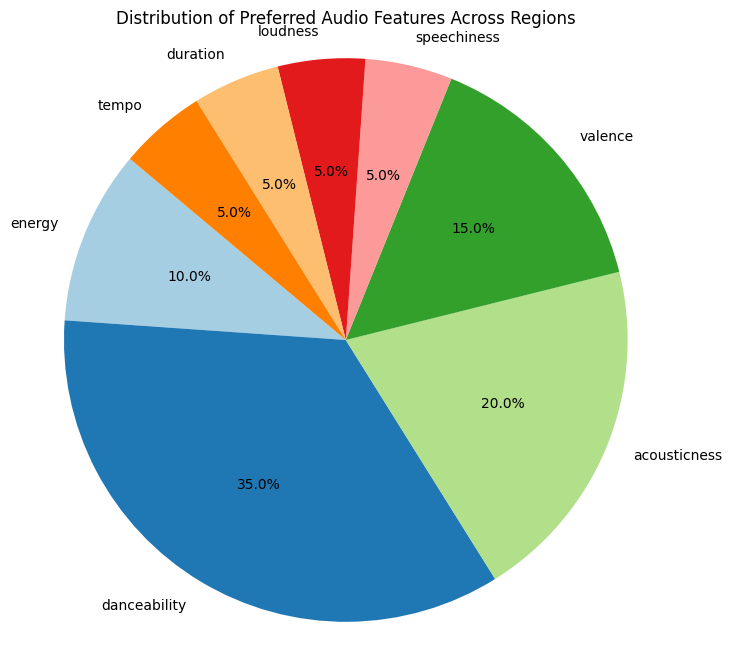
\includegraphics[width=\linewidth]{media/features_preferences.png}
        \caption{Global Feature Importance}
    \end{minipage}%
    \hspace{0.05\textwidth} % Space between the two figures
    \begin{minipage}{0.45\textwidth}
        \centering
        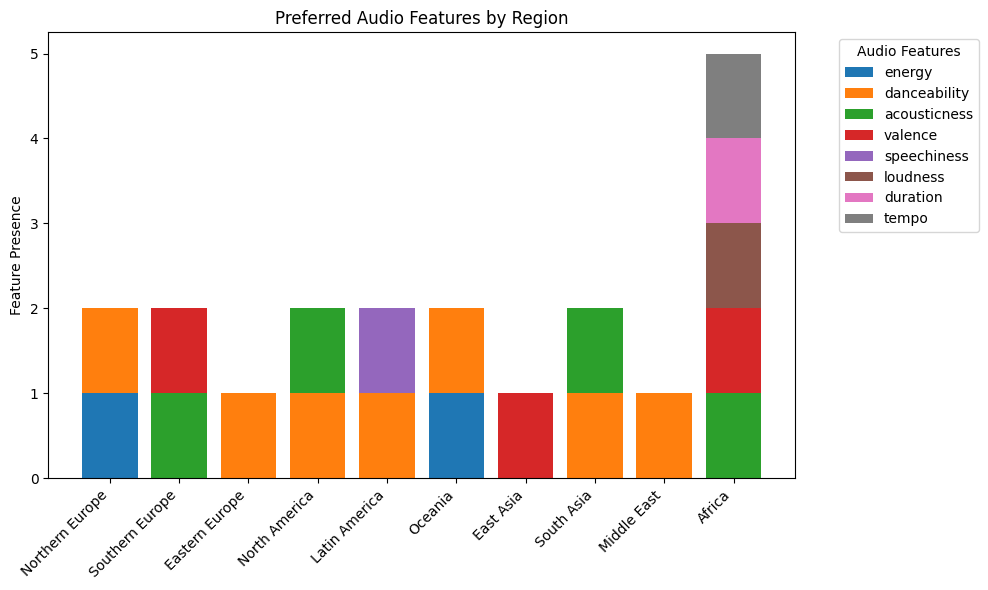
\includegraphics[width=\linewidth]{media/feature_preferences_regions.png}
        \caption{Regional Feature Importance}
    \end{minipage}
\end{figure}